\chapter{Acoustic emissions}

Modeling the acoustic emissions is a core feature of APECSS. To this end, APECSS offers different models for the acoustic emissions, assuming an incompressible liquid, a weakly-compressible liquid or a fully-compressible liquid. To account for a finite propagation speed, the information associated with an emitted acoustic wave is propagated along the radial coordinate axis using a Lagrangian wave tracking approach. Please refer to the work of \citet{Denner2023} for a detailed explanation and validation of the different emission models. Unless specifically told to do so, APECSS does not compute any acoustic emissions. 

\vspace{0.8em}

\noindent
\begin{tabular}{p{0.1\textwidth} p{0.32\textwidth} p{0.5\textwidth}}
    \textbf{Section} &\textbf{Command} & \textbf{Description} 
\vspace{1mm} \\ \hline
{\tt BUBBLE} & {\tt Emissions IC <float>} & Computes the acoustic emissions using the standard incompressible model, Section \ref{sec:emissionsic}.\\ 
& {\tt Emissions FSIC <float>} & Computes the acoustic emissions using the finite-speed incompressible model, Section \ref{sec:emissionsfsic}.\\ 
& {\tt Emissions QA <float>} & Computes the acoustic emissions using the quasi-acoustic model, Section \ref{sec:emissionsqa}.\\ 
& {\tt Emissions EV <float>} & Computes the acoustic emissions based on the Kirkwood-Bethe hypothesis, Section \ref{sec:emissionskb}, with the explicit expression for velocity, see Eq.~\eqref{eq:u_rt}.\\ 
& {\tt Emissions TIV <float>} & Computes the acoustic emissions using the model of \citet{Hickling1963} based on the Kirkwood-Bethe hypothesis, Section \ref{sec:emissionskb}, with the temporally-integrated velocity, see Eq.~\eqref{eq:dudt_rt}.\\ 
& {\tt EmissionIntegration Euler} & Integrates the radial position and, if applicable, the velocity using an Euler scheme.\\
& {\tt EmissionIntegration RK4} & Integrates the radial position and, if applicable, the velocity using a conventional fourth-order Runge-Kutta scheme. This is the default.\\
& {\tt KBIterTolerance <float>} & Tolerance $\eta$ for the evaluation of the pressure using a model based on the Kirkwood-Bethe hypothesis in conjunction with the NASG EoS.\\
 \hline
\end{tabular} \vspace{0.2em}

The floating-point value given as the final argument of the {\tt Emissions} command defines the cut-off distance beyond which the emissions are not computed. For the standard incompressible assumption this value has no meaning, but a value is required as a dummy to facilitate the correct reading of the options.

\section{Lagrangian wave tracking}

APECSS tracks acoustic emissions using a Lagrangian wave tracking approach \citep{Denner2023}, illustrated in Figure \ref{fig:lagrangiantracking}, in which so-called \textit{emission nodes} are propagated in the radial direction with propagation speed $\mathcal{C}$. Each emission node, represented in APECSS as a structure {\tt struct APECSS\_EmissionNode} and part of a linked list of these structures, holds the current radial coordinate $r(t)$, the flow velocity $u(r,t)$, the pressure $p(r,t$) and, if applicable, the enthalpy $h(r,t)$, as well as the invariants $f(\tau)$ and $g(\tau)$ computed based on the solution of the RP model. The radial position of an emission node at time $t$ is given as
\begin{equation}
    r(t) = R(\tau) + \int_\tau^t \mathcal{C}(r,t) \, \mathrm{d}t, 
    \label{eq:r_t}
\end{equation}
In general, the propagation speed is defined by $\mathcal{C}=c+u$, but the actual value used depends on the chosen model.

\begin{figure}
    \begin{center}
    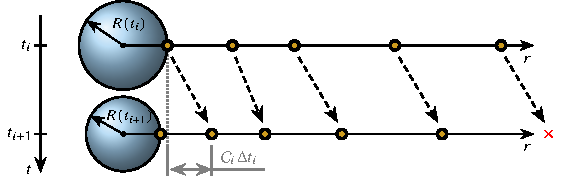
\includegraphics[width=0.7\linewidth]{LagrangianWaveTracking.pdf}
    \caption{Illustration of the Lagrangian transport of the emission nodes, updated at each discrete time instance $t_i$. Nodes that pass a predefined maximum radial coordinate are discarded.}
    \label{fig:lagrangiantracking}
    \end{center}
\end{figure}

\section{Standard incompressible model}
\label{sec:emissionsic}

Assuming an incompressible liquid ($c_{\ell,\mathrm{ref}} \rightarrow  \infty$) with density $\rho_{\ell,\mathrm{ref}}$, the velocity $u(r,t)$ and pressure $p(r,t)$ at a given radial position $r(t)$ are defined as \citep{Neppiras1980}
\begin{equation}
    u(r,t) = \frac{R(t)^2 \dot{R}(t)}{r^2}  \label{eq:u_rt_incomp} 
\end{equation}
and 
\begin{equation}
    p(r,t) = p_\infty(t) + \rho_{\ell,\mathrm{ref}} \left[\frac{R(t)^2 \, \ddot{R}(t) + 2 \, R(t) \, \dot{R}(t)^2}{r} - \frac{R(t)^4 \, \dot{R}(t)^2}{2 \, r^4} \right], \label{eq:p_rt_incomp}
\end{equation}
respectively. The assumption of an incompressible fluid is consistent with the Rayleigh-Plesset models in Eqs.~\eqref{eq:standardRP} and \eqref{eq:modRP}. Note that, because $\mathcal{C} \rightarrow \infty$, these simple incompressible acoustic emissions do not use the Lagrangian wave tracking and no emission nodes are defined and processed, since pressure and velocity are defined instantaneously for all $r$.

\section{Quasi-acoustic model}
\label{sec:emissionsqa}

Assuming the liquid is compressible but accurately described by a constant density $\rho_{\ell,\mathrm{ref}}$ and constant speed of sound $c_{\ell,\mathrm{ref}}$, with $u \ll c_{\ell,\mathrm{ref}}$ and $\mathcal{C} = c_{\ell,\mathrm{ref}}$, \citet{Trilling1952} and \citet{Gilmore1952} derived the {\it quasi-acoustic model} for the acoustic emissions. With the quasi-acoustic model, the velocity, pressure and radial position follow as
\begin{align}
    u(r,t) &= \frac{f(\tau)}{r(t)^2} + \frac{g(\tau)}{r(t) \, c_{\ell,\mathrm{ref}}}  \label{eq:u_rt_qa} \\
  p(r,t) &=  p_\infty(t) + \rho_{\ell,\mathrm{ref}} \left[ \frac{g(\tau)}{r(t)} - \frac{u(r,t)^2}{2} \right] \label{eq:p_rt_qa} \\
  r(t) &\approx R(\tau) + c_{\ell,\mathrm{ref}} \sum_{i=1}^N \Delta t_{i-1}, \label{eq:r_t_qa}
\end{align}
where $f(\tau)$ and $g(\tau)$ are invariants defined based on the result of the employed RP model as
\begin{align}
    f(\tau) &= R(\tau)^2 \dot{R}(\tau) - \frac{R(\tau) g(\tau)}{c_{\ell,\mathrm{ref}}}\\
    g(\tau) &= R(\tau) \left[\frac{p_\mathrm{L}(\tau)-p_\infty(\tau)}{\rho_{\ell,\mathrm{ref}}} + \frac{\dot{R}(\tau)^2}{2} \right], \label{eq:g_qa}
\end{align}
and $\tau$ is the time at which the acoustic information is emitted at the bubble wall. For $t=\tau$ with $r(t)=R(\tau)$, Eq.~(\ref{eq:u_rt_qa}) reduces to $u(R,\tau)=\dot{R}(\tau)$ and Eq.~(\ref{eq:p_rt_qa}) reduces to $p(R,\tau)=p_\mathrm{L}(\tau)$, thus satisfying the boundary conditions at the bubble wall. 

The quasi-acoustic model is consistent in its modelling assumptions with the Keller-Miksis model, Eq.~\eqref{eq:keller}. The applicability of the quasi-acoustic model is limited to small Mach numbers, $(\dot{R}/c_0)^2 \ll 1$, as it incorporates a finite propagation speed of the acoustic emissions and the nonlinear pressure contributions resulting from the flow, but since all parts of the wave propagate with speed $c_0$, the quasi-acoustic model can neither describe the nonlinear distortion of acoustic waves nor the formation of shock fronts. 

\section{Finite-speed incompressible model}
\label{sec:emissionsfsic}

APECSS also supports the assumption that the liquid is incompressible but the information associated with the acoustic emissions still propagates with finite speed $\mathcal{C} = c_{\ell,\mathrm{ref}}$ using the Lagrangian wave tracking approach, with the radial location given by Eq.~\eqref{eq:r_t_qa}.
By assuming the specific acoustic impedance of an incompressible liquid, $\rho_{\ell,\mathrm{ref}} c_{\ell,\mathrm{ref}} \rightarrow \infty$, the velocity reduces to
\begin{align}
    u(r,t) = \frac{R(\tau)^2 \dot{R}(\tau)}{r(t)^2}, \label{eq:u_rt_fsic} 
\end{align}
while $p(r,t)$ and $g(\tau)$ are given by Eq.~\eqref{eq:p_rt_qa} and Eq.~\eqref{eq:g_qa}, respectively.
This approach, referred to in APECSS as {\tt FSIC} or \text{finite-speed incompressible model}, recovers the time delay between emitting information at the bubble wall and this information arriving in a certain location, but treats the flow field as incompressible.

\section{Emissions based on the Kirkwood-Bethe hypothesis}
\label{sec:emissionskb}

Under the Kirkwood-Bethe hypothesis \citep{Kirkwood1942,Cole1948}, the propagation speed along the outgoing characteristic is given as $\mathcal{C}(r,t) = c(r,t) + u(r,t)$. The ODE describing the radial position along the outgoing characteristics is, thus, defined as 
\begin{equation}
    \left. \frac{\mathrm{d}r(t)}{\mathrm{d}t} \right|_\text{c} = c(r,t) + u(r,t). \label{eq:drdt}
\end{equation}
This ODE is numerically integrated using either an Euler scheme or a fourth-order Runge-Kutta (RK4) scheme, with initial condition $r(t) = R(\tau)$ for $t=\tau$, where $\tau$ is the time at which the acoustic information is emitted at the bubble wall. The time-step $\Delta t$ is taken to be the same as used for the integration of the model describing the bubble dynamics (see Section \ref{chap:bubble}).

Two models to compute the velocity $u(r,t)$ at a given emission node are available in APECSS: (i) an explicit expression for $u(r,t)$ \citep{Denner2023}  and (ii) integrating the temporal derivative of the velocity, $\mathrm{d}u(r,t)/\mathrm{d}t$, along the outgoing characteristic, as proposed by \citet{Hickling1963}. The assumptions used to derive these models for the acoustic emissions are consistent with the Gilmore model, Eq.~\eqref{eq:gilmore}.

Following a similar derivation as for the quasi-acoustic model discussed in Section \ref{sec:emissionsqa}, but assuming a fully-compressible liquid described by a suitable equation of state, the {\it explicit velocity (EV)} is given as
\begin{equation}
    u(r,t) = \frac{f(\tau)}{r(t)^2} + \frac{g(\tau)}{r(t) \, [c(r,t) + u(r,t)]} , \label{eq:u_rt}
\end{equation}
with 
\begin{equation}
    f(\tau) = R(\tau)^2 \dot{R}(\tau) - \frac{R(\tau) \, g(\tau)}{c_\mathrm{L}(\tau) + \dot{R}(\tau)}  . \label{eq:f_R}
\end{equation}
For $t=\tau$ with $r(t)=R(\tau)$, this expression reduces to $u(R,\tau)=\dot{R}(\tau)$, thus satisfying the boundary conditions at the bubble wall.

\citet{Hickling1963} proposed to integrate the velocity with respect to time, in APECSS referred to as {\it temporally-integrated velocity (TIV)}, with the temporal derivative of the velocity along the outgoing characteristic given as
\begin{equation}
    \left. \frac{\mathrm{d}u(r,t)}{\mathrm{d}t} \right|_\text{c} =  - \frac{2 c(r,t)^2 u(r,t)}{r(t) \, [c(r,t)-u(r,t)]} + \frac{g(\tau)}{r(t)^2} \, \frac{c(r,t)+u(r,t)}{c(r,t)-u(r,t)}. \label{eq:dudt_rt}
\end{equation}
This differential equation for the velocity is integrated together with the equation for ${\mathrm{d}r(t)/\mathrm{d}t}$, Eq.~\eqref{eq:drdt}, using the initial condition $u(R,\tau) = \dot{R}(\tau)$. 

Regardless of the choice of velocity model, the invariant $g(\tau)$ is defined as
\begin{align}
    g(\tau) = R(\tau) \left[h_\mathrm{L}(\tau) - h_\infty(\tau) + \frac{\dot{R}(\tau)^2}{2} \right]
    \label{eq:g_R} .
\end{align}
For a given radial position $r(t)$ and flow velocity $u(r,t)$, irrespective of which model is used to compute the velocity, the enthalpy is readily evaluated as
\begin{equation}
    h(r,t) = h_\infty(t) + \frac{g(\tau)}{r(t)} - \frac{u(r,t)^2}{2}, \label{eq:h_rt}
\end{equation}
where $h_\infty$ is spatially invariant and only depends on time. For $t=\tau$ with $r(t)=R(\tau)$, this expression for enthalpy reduces to $h(R,\tau)=h_\mathrm{L}(\tau)$, satisfying the boundary conditions at the bubble wall. 

Using the Tait EoS, the pressure can be readily computed from the enthalpy defined in Eq.~(\ref{eq:h_rt}) by inserting Eq.~(\ref{eq:rho_Tait}) into Eq.~(\ref{eq:h_Tait}) and rearranging to yield
\begin{equation}
    p(r,t) = \left[ \frac{(\Gamma-1) \, \rho_0}{\Gamma \, (p_0+B)^{1/\Gamma}} \, h(r,t) \right]^{\frac{1}{1-1/\Gamma}} - B. \label{eq:p_rt}
\end{equation}
Solving Eq.~(\ref{eq:p_rt}) is straightforward because the enthalpy $h(r,t)$ is the only variable, all other quantities are predefined fluid properties. Using the NASG EoS, pressure $p(r,t)$ follows by rearranging Eq.~(\ref{eq:h_NASG}) as
\begin{eqnarray}
p(r,t) = \frac{\left[\Gamma-1\right] \rho(r,t) \, h(r,t) - \left[1 - b \, \rho(r,t) \right] \Gamma B}{\Gamma - b \, \rho(r,t)}.  \label{eq:p_rt_NASG}
\end{eqnarray}
Since the pressure $p(r,t)$ and the density $\rho(r,t)$ depend explicitly on each other in this formulation, Eq.~(\ref{eq:p_rt_NASG}) has to be solved iteratively. As a convergence criterion for the iterative approximation we use $|p_j(r,t) - p_{j-1}(r,t)| < \eta \, |p_j(r,t)|$, where $j$ denotes the iteration counter and $\eta$ is a predefined tolerance (see option {\tt KBIterTolerance}). Preliminary tests identified a tolerance of $\eta = 10^{-4}$ to be sufficiently small.

Emission nodes with a higher pressure propagate faster than nodes with a lower pressure, which in turn leads to progressive steepening of the acoustic wave. As a result, an emission node may overtake the forerunning emission node, yielding an unphysical multivalued solution. In reality, such a multivalued solution is avoided by the formation of a shock front \citep{Fay1931}. While treating such multivalued solutions is often done in a post-processing step, APECSS deals with multivalued solutions at run time. An emission node that overtakes its forerunning neighbor is discarded, see Fig.~\ref{fig:lagrangiantrackingshock}, and the thermodynamic values of the forerunning neighbor are reevaluated by a simple averaging procedure. Thus, a unique and physically plausible solution is maintained.

\begin{figure}
    \begin{center}
    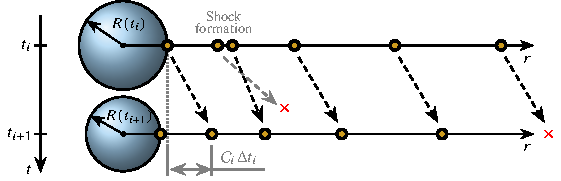
\includegraphics[width=0.7\linewidth]{LagrangianWaveTracking_withShock.pdf}
    \caption{Illustration of the Lagrangian transport of the emission nodes, updated at each discrete time instance $t_i$. Nodes that either overtake the forerunning node, which represents the formation of a shock front, or that pass a predefined maximum radial coordinate are discarded.}
    \label{fig:lagrangiantrackingshock}
    \end{center}
\end{figure}


\section{Results}
\label{sec:emissions_results}

APECSS can write out different results based on the acoustic emissions. Note that APECSS does \uline{not} write any results to disk unless it is specifically ask to do so.

The acoustic emissions can be recorded as a function of time at one or multiple radial locations (cf.~{\tt EmissionsSpace}), or the emissions are written out with respect to their radial location at one or multiple time instances (cf.~{\tt EmissionsTime}) or emission nodes (cf.~{\tt EmissionsNode}), or for selected extrema in a specified period (cf.~{\tt EmissionsMinMax}). This calls can be used multiple times to defined, for instance, multiple radial locations or time instances.

\vspace{0.8em}

\noindent
\begin{tabular}{p{0.1\textwidth} p{0.36\textwidth} p{0.49\textwidth}}
    \textbf{Section} &\textbf{Command} & \textbf{Description} 
\vspace{1mm} \\ \hline
{\tt RESULTS} & {\tt OutputPath <string>} & Path to the folder where all the results should be written in to (default: {\tt ./}).\\
& {\tt OutputDigits <int>} & Results are written out with as many digits (default: 6).\\
& {\tt EmissionsSpace <float>} & Defines a radial location at which the emissions in the liquid are written out as a function of time. If/while the location is in the gas phase, $0$ is recorded.\\ 
& {\tt OutputFreqEmissionsSpace <int>} & Results of the emissions at a specific radial location are stored every so many time steps (default: 1).\\ 
& {\tt EmissionsTime <float>} & Defines a time instance at which the emission in the liquid are written out as a function of the radial coordinate.\\ 
& {\tt EmissionsNode <int>} & Defines a node ID of which the emission in the liquid are written out as a function of the radial coordinate.\\ 
& {\tt EmissionsMinMax <int>} & Defines the period in which the emission in the liquid are written out as a function of the radial coordinate for the node representing $R_\mathrm{min}$, $\dot{R}_\mathrm{min}$ and $p_\mathrm{L,max}$.\\ 
 \hline
\end{tabular}

The first line of the results file(s) lists the variables that were written out and their order. For instance, Figure \ref{fig:emissions_results} shows the different ways in which emissions can be recorded, using the sonoluminescence example found in the {\tt \$APECSS\_DIR/examples/ultrasound/} folder.

\begin{figure}
    \centering
    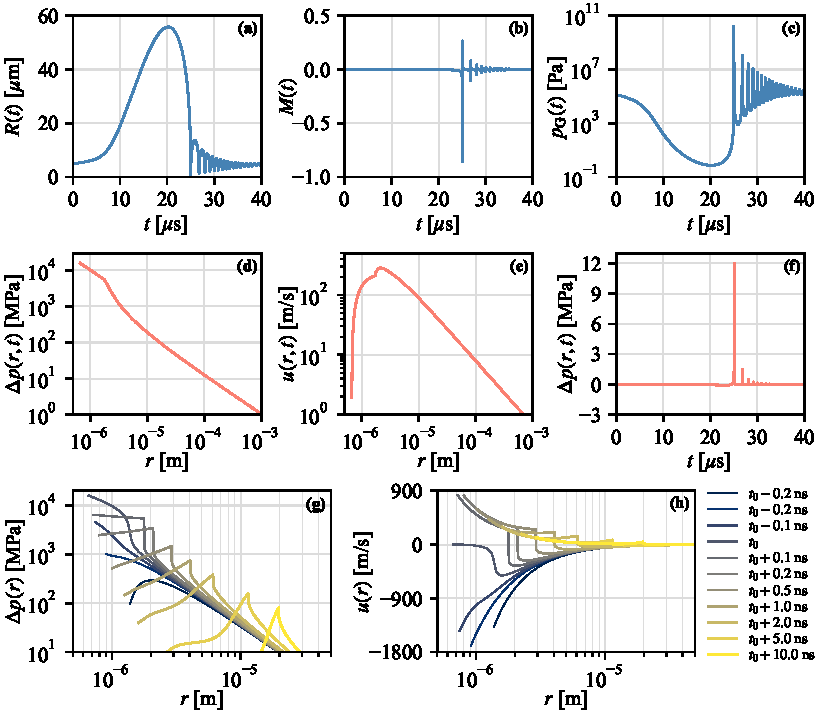
\includegraphics[width=\linewidth]{./figures/emissions_results.pdf}
    \caption{Results of an argon bubble with initial radius $R_0 = 5 \, \upmu \mathrm{m}$ in water, driven by ultrasound with a frequency of $23.5 \, \mathrm{kHz}$ and a pressure amplitude of $145 \, \mathrm{kPa}$, as previously considered by \citet{Holzfuss2010}. {\bf(a)}-{\bf(c)} The bubble radius $R(t)$, bubble-wall Mach number $M(t)=\dot{R}(t)/c_\mathrm{L}(t)$, and gas pressure $p_\mathrm{G}(t)$ as a function of time $t$. {\bf(d)}-{\bf(e)} The pressure amplitude $\Updelta p(r,t)$ and velocity $u(r,t)$  of the acoustic wave generated by the primary collapse of the bubble as a function of the radial coordinate $r$. {\bf (f)} The pressure amplitude $\Updelta p(r,t)$ emitted by the bubble at a fixed radial distance $r=100 \, \upmu \mathrm{m}$ from the bubble center as a function of time $t$. {\bf(g)}-{\bf(h)} Spatial profiles of the pressure amplitude $\Delta p(r,t)$ and the velocity $u(r,t)$ at selected time instances, where $t_0$ is the time at which the bubble assumes its minimum radius. This example can be found in {\tt \$APECSS\_DIR/examples/ultrasound}, called {\tt sonolum\_emissions}.}
    \label{fig:emissions_results}
\end{figure}